

\PassOptionsToPackage{unicode=true}{hyperref} % options for packages loaded elsewhere
\PassOptionsToPackage{hyphens}{url}
\PassOptionsToPackage{dvipsnames,svgnames*,x11names*}{xcolor}
%
\documentclass[]{book}
\usepackage{lmodern}
\usepackage{amssymb,amsmath}
\usepackage{ifxetex,ifluatex}
\usepackage{fixltx2e} % provides \textsubscript
\ifnum 0\ifxetex 1\fi\ifluatex 1\fi=0 % if pdftex
  \usepackage[T1]{fontenc}
  \usepackage[utf8]{inputenc}
  \usepackage{textcomp} % provides euro and other symbols
\else % if luatex or xelatex
  \usepackage{unicode-math}
  \defaultfontfeatures{Ligatures=TeX,Scale=MatchLowercase}
\fi
% use upquote if available, for straight quotes in verbatim environments
\IfFileExists{upquote.sty}{\usepackage{upquote}}{}
% use microtype if available
\IfFileExists{microtype.sty}{%
\usepackage[]{microtype}
\UseMicrotypeSet[protrusion]{basicmath} % disable protrusion for tt fonts
}{}
\IfFileExists{parskip.sty}{%
\usepackage{parskip}
}{% else
\setlength{\parindent}{0pt}
\setlength{\parskip}{6pt plus 2pt minus 1pt}
}
\usepackage{xcolor}
\usepackage{hyperref}
\hypersetup{
            pdftitle={The Open Quant Live Book},
            pdfauthor={Thársis T. P. Souza},
            colorlinks=true,
            linkcolor=Maroon,
            filecolor=Maroon,
            citecolor=Blue,
            urlcolor=Blue,
            breaklinks=true}
\urlstyle{same}  % don't use monospace font for urls
\usepackage{geometry}
\geometry{paperwidth=6in, paperheight=9in}
\usepackage{color}
\usepackage{fancyvrb}
\newcommand{\VerbBar}{|}
\newcommand{\VERB}{\Verb[commandchars=\\\{\}]}
\DefineVerbatimEnvironment{Highlighting}{Verbatim}{commandchars=\\\{\}}
% Add ',fontsize=\small' for more characters per line
\usepackage{framed}
\definecolor{shadecolor}{RGB}{248,248,248}
\newenvironment{Shaded}{\begin{snugshade}}{\end{snugshade}}
\newcommand{\KeywordTok}[1]{\textcolor[rgb]{0.13,0.29,0.53}{\textbf{#1}}}
\newcommand{\DataTypeTok}[1]{\textcolor[rgb]{0.13,0.29,0.53}{#1}}
\newcommand{\DecValTok}[1]{\textcolor[rgb]{0.00,0.00,0.81}{#1}}
\newcommand{\BaseNTok}[1]{\textcolor[rgb]{0.00,0.00,0.81}{#1}}
\newcommand{\FloatTok}[1]{\textcolor[rgb]{0.00,0.00,0.81}{#1}}
\newcommand{\ConstantTok}[1]{\textcolor[rgb]{0.00,0.00,0.00}{#1}}
\newcommand{\CharTok}[1]{\textcolor[rgb]{0.31,0.60,0.02}{#1}}
\newcommand{\SpecialCharTok}[1]{\textcolor[rgb]{0.00,0.00,0.00}{#1}}
\newcommand{\StringTok}[1]{\textcolor[rgb]{0.31,0.60,0.02}{#1}}
\newcommand{\VerbatimStringTok}[1]{\textcolor[rgb]{0.31,0.60,0.02}{#1}}
\newcommand{\SpecialStringTok}[1]{\textcolor[rgb]{0.31,0.60,0.02}{#1}}
\newcommand{\ImportTok}[1]{#1}
\newcommand{\CommentTok}[1]{\textcolor[rgb]{0.56,0.35,0.01}{\textit{#1}}}
\newcommand{\DocumentationTok}[1]{\textcolor[rgb]{0.56,0.35,0.01}{\textbf{\textit{#1}}}}
\newcommand{\AnnotationTok}[1]{\textcolor[rgb]{0.56,0.35,0.01}{\textbf{\textit{#1}}}}
\newcommand{\CommentVarTok}[1]{\textcolor[rgb]{0.56,0.35,0.01}{\textbf{\textit{#1}}}}
\newcommand{\OtherTok}[1]{\textcolor[rgb]{0.56,0.35,0.01}{#1}}
\newcommand{\FunctionTok}[1]{\textcolor[rgb]{0.00,0.00,0.00}{#1}}
\newcommand{\VariableTok}[1]{\textcolor[rgb]{0.00,0.00,0.00}{#1}}
\newcommand{\ControlFlowTok}[1]{\textcolor[rgb]{0.13,0.29,0.53}{\textbf{#1}}}
\newcommand{\OperatorTok}[1]{\textcolor[rgb]{0.81,0.36,0.00}{\textbf{#1}}}
\newcommand{\BuiltInTok}[1]{#1}
\newcommand{\ExtensionTok}[1]{#1}
\newcommand{\PreprocessorTok}[1]{\textcolor[rgb]{0.56,0.35,0.01}{\textit{#1}}}
\newcommand{\AttributeTok}[1]{\textcolor[rgb]{0.77,0.63,0.00}{#1}}
\newcommand{\RegionMarkerTok}[1]{#1}
\newcommand{\InformationTok}[1]{\textcolor[rgb]{0.56,0.35,0.01}{\textbf{\textit{#1}}}}
\newcommand{\WarningTok}[1]{\textcolor[rgb]{0.56,0.35,0.01}{\textbf{\textit{#1}}}}
\newcommand{\AlertTok}[1]{\textcolor[rgb]{0.94,0.16,0.16}{#1}}
\newcommand{\ErrorTok}[1]{\textcolor[rgb]{0.64,0.00,0.00}{\textbf{#1}}}
\newcommand{\NormalTok}[1]{#1}
\usepackage{longtable,booktabs}
% Fix footnotes in tables (requires footnote package)
\IfFileExists{footnote.sty}{\usepackage{footnote}\makesavenoteenv{longtable}}{}
\usepackage{graphicx,grffile}
\makeatletter
\def\maxwidth{\ifdim\Gin@nat@width>\linewidth\linewidth\else\Gin@nat@width\fi}
\def\maxheight{\ifdim\Gin@nat@height>\textheight\textheight\else\Gin@nat@height\fi}
\makeatother
% Scale images if necessary, so that they will not overflow the page
% margins by default, and it is still possible to overwrite the defaults
% using explicit options in \includegraphics[width, height, ...]{}
\setkeys{Gin}{width=\maxwidth,height=\maxheight,keepaspectratio}
% Make links footnotes instead of hotlinks:
\DeclareRobustCommand{\href}[2]{#2\footnote{\url{#1}}}
\setlength{\emergencystretch}{3em}  % prevent overfull lines
\providecommand{\tightlist}{%
  \setlength{\itemsep}{0pt}\setlength{\parskip}{0pt}}
\setcounter{secnumdepth}{5}
% Redefines (sub)paragraphs to behave more like sections
\ifx\paragraph\undefined\else
\let\oldparagraph\paragraph
\renewcommand{\paragraph}[1]{\oldparagraph{#1}\mbox{}}
\fi
\ifx\subparagraph\undefined\else
\let\oldsubparagraph\subparagraph
\renewcommand{\subparagraph}[1]{\oldsubparagraph{#1}\mbox{}}
\fi

% set default figure placement to htbp
\makeatletter
\def\fps@figure{htbp}
\makeatother

\usepackage{booktabs}
\usepackage{amsthm}
\usepackage{pdfpages}
\usepackage{graphicx}
\usepackage[]{natbib}
\bibliographystyle{apalike}

\title{The Open Quant Live Book}
\author{Thársis T. P. Souza}
\date{2019-01-04}

\let\BeginKnitrBlock\begin \let\EndKnitrBlock\end
\begin{document}

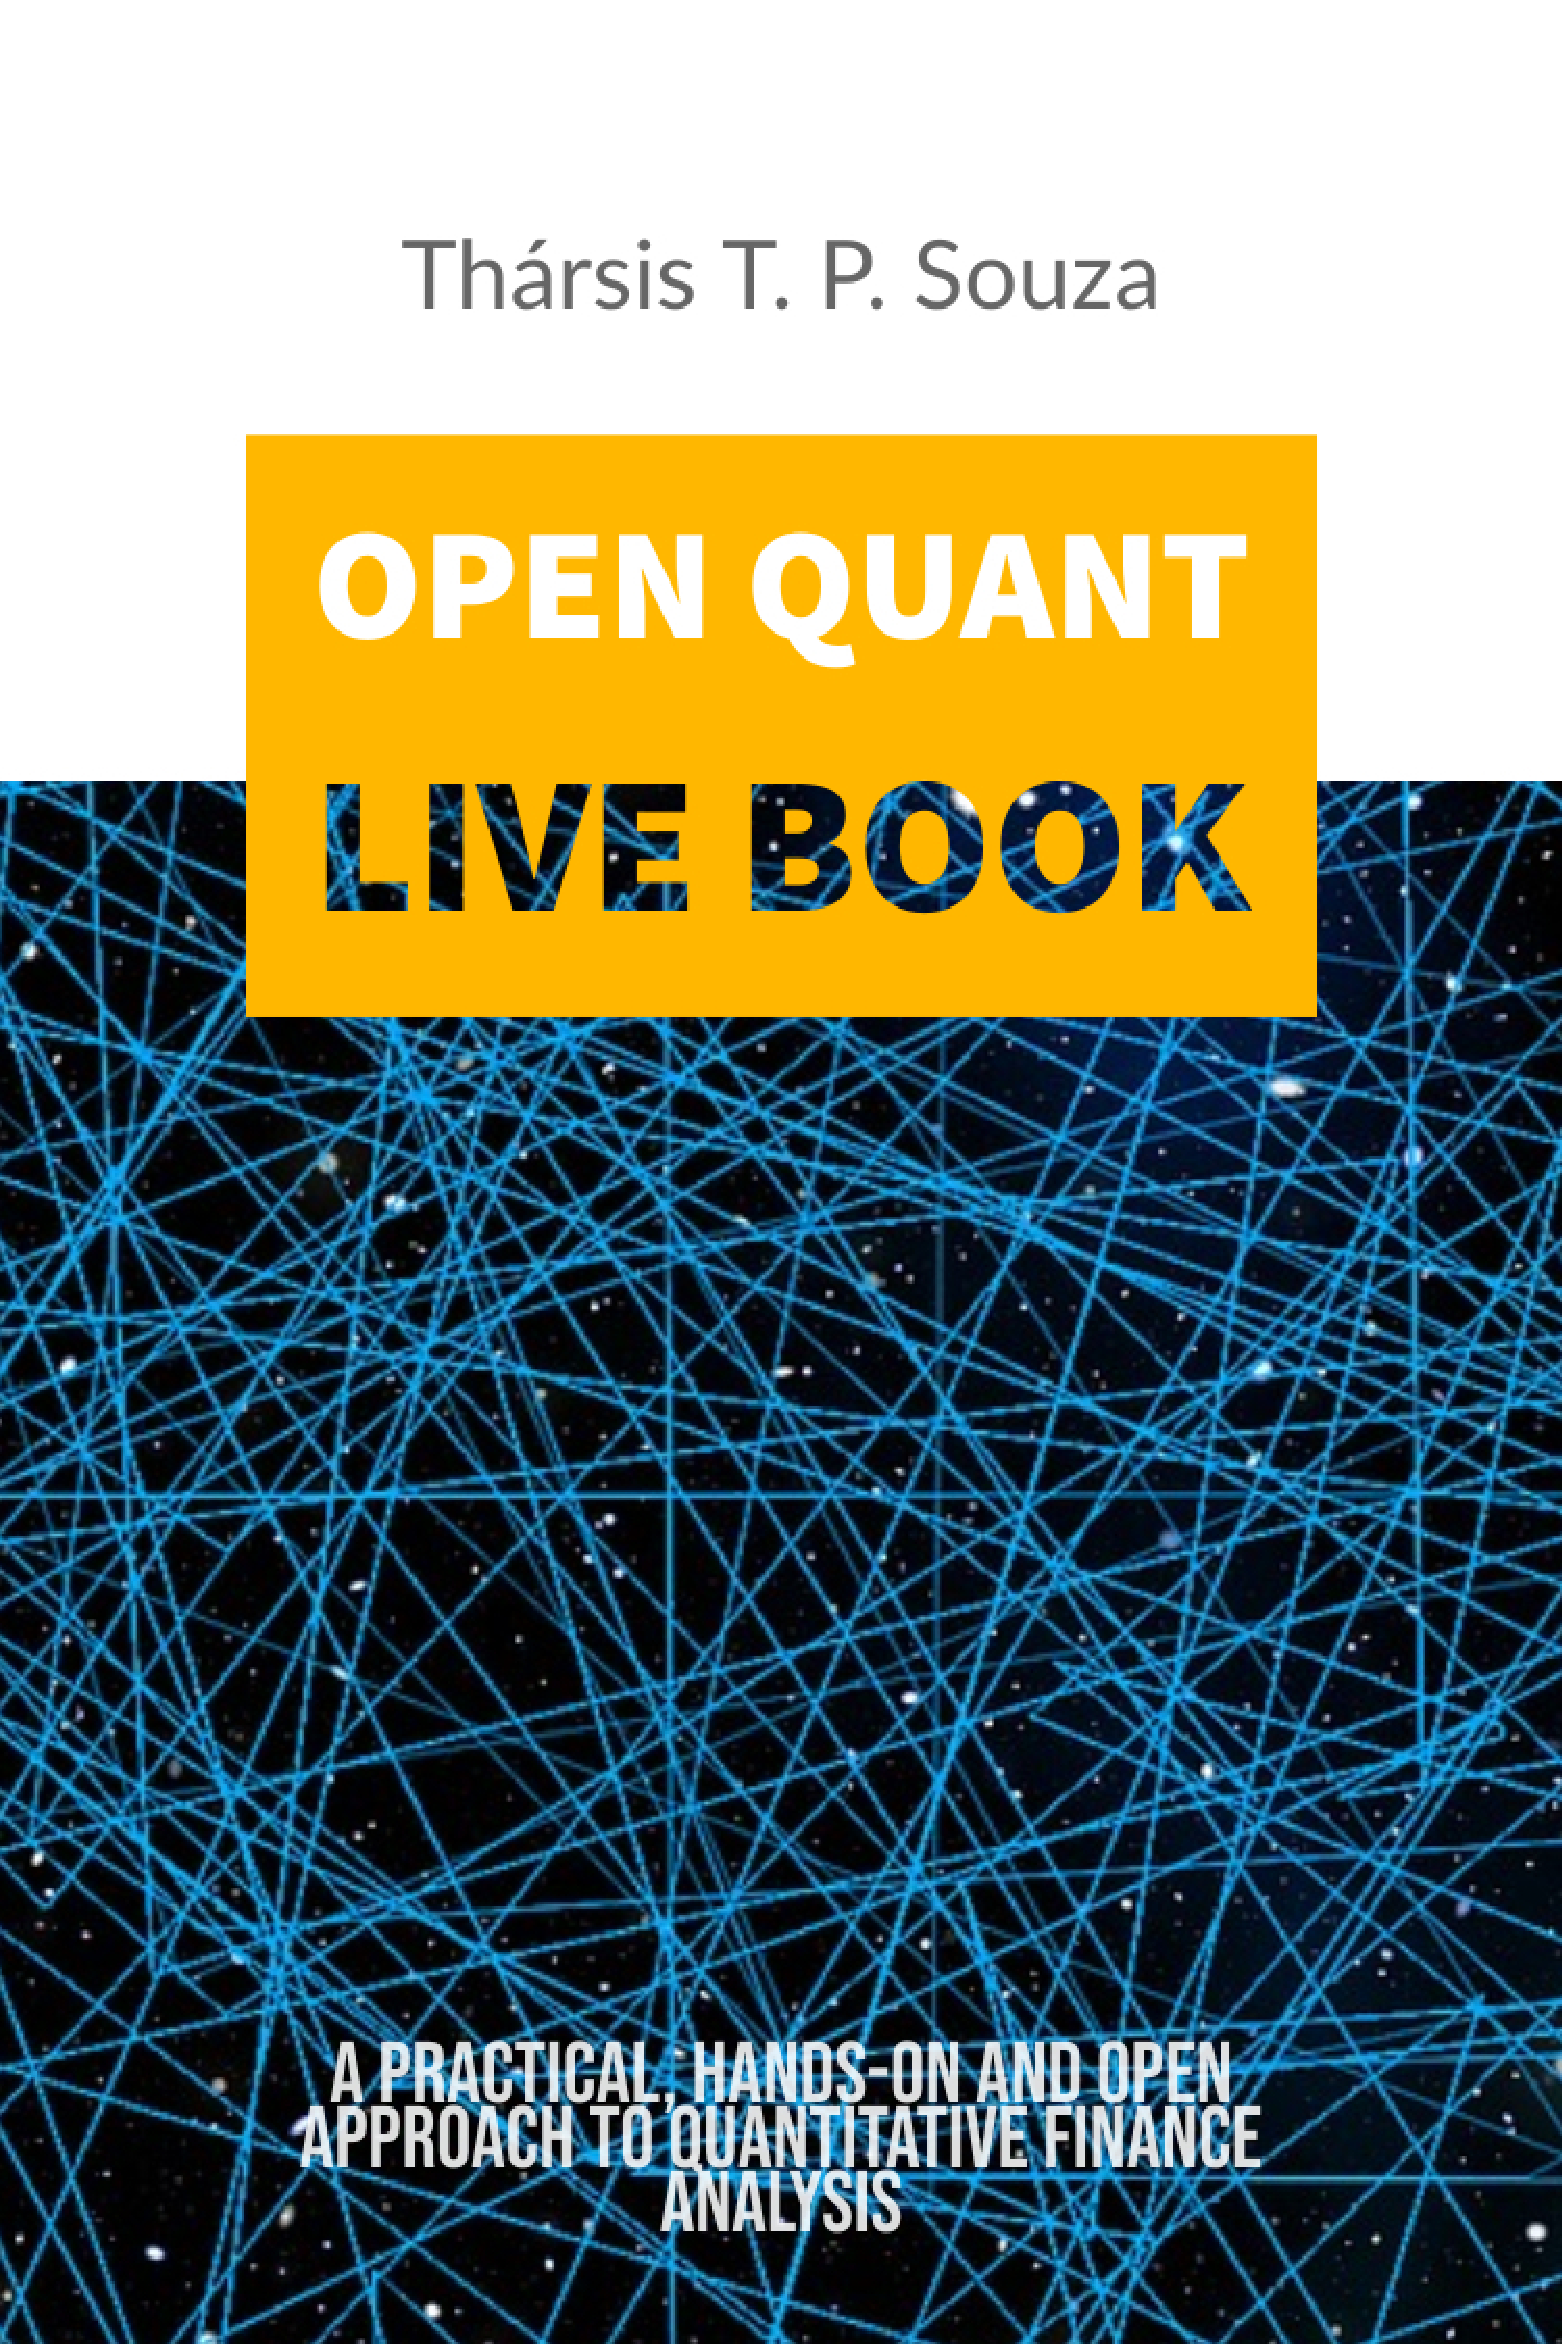
\includepdf{./fig/cover1.pdf}

\maketitle

{
\hypersetup{linkcolor=}
\setcounter{tocdepth}{2}
\tableofcontents
}
\chapter*{Preface}\label{preface}


\subsection*{Working Contents}\label{working-contents}


\begin{enumerate}
\def\labelenumi{\arabic{enumi}.}
\tightlist
\item
  The Basics
\end{enumerate}

\begin{itemize}
\tightlist
\item
  I/O
\item
  Stylized Facts
\item
  Correlation \& Causation
\end{itemize}

\begin{enumerate}
\def\labelenumi{\arabic{enumi}.}
\setcounter{enumi}{1}
\tightlist
\item
  Algo Trading
\end{enumerate}

\begin{itemize}
\tightlist
\item
  Investment Process
\item
  Backtesting
\item
  Factor Investing
\item
  Limit Order
\end{itemize}

\begin{enumerate}
\def\labelenumi{\arabic{enumi}.}
\setcounter{enumi}{2}
\tightlist
\item
  Portfolio Optimization
\end{enumerate}

\begin{itemize}
\tightlist
\item
  Modern Portfolio Theory
\item
  Measuring Risk
\item
  Linear Programming
\end{itemize}

\begin{enumerate}
\def\labelenumi{\arabic{enumi}.}
\setcounter{enumi}{3}
\tightlist
\item
  Machine Learning
\end{enumerate}

\begin{itemize}
\tightlist
\item
  Intro
\item
  Agent-Based Models
\item
  Binary Classifiers
\item
  AutoML
\item
  Hierarchical Risk Parity
\end{itemize}

\begin{enumerate}
\def\labelenumi{\arabic{enumi}.}
\setcounter{enumi}{4}
\tightlist
\item
  Econophysics
\end{enumerate}

\begin{itemize}
\tightlist
\item
  Entropy, Efficiency and Coupling
\item
  Transfer Entropy, Information Transfer and Causality
\item
  Financial Networks
\end{itemize}

\begin{enumerate}
\def\labelenumi{\arabic{enumi}.}
\setcounter{enumi}{5}
\tightlist
\item
  Alternative Data
\end{enumerate}

\subsection*{Contribute}\label{contribute}


The Book is
\href{https://github.com/souzatharsis/open-quant-live-book}{Open} and we
are looking for co-authors. Feel free to
\href{http://www.souzatharsis.com/}{reach out} or simply create a pull
request with your contribution on our
\href{https://github.com/souzatharsis/open-quant-live-book}{Github
project}.

\subsection*{Book's information}\label{books-information}


First published at:
\href{https://openquant.netlify.com/}{openquant.netlify.com}.

Licensed under
\href{https://creativecommons.org/licenses/by-nc-sa/4.0/}{Attribution-NonCommercial-ShareAlike
4.0 International}.


\includegraphics[width=0.2\linewidth]{fig/by-nc-sa}

\BeginKnitrBlock{flushright}
Copyright (c) 2018. Thársis T. P. Souza. New York, NY.
\EndKnitrBlock{flushright}

\part{The Basics}\label{part-the-basics}

\chapter{I/O}\label{io}

In this Chapter, we will introduce basic input and output functions in
R. You will learn how to read text and excel files as well as how to
read large files. We will also show how to obtain free financial and
economic data from sources such as Quandl, IEX and Alpha Vantage.

\section{Reading and Writing}\label{reading-and-writing}

\subsection{Text Files}\label{text-files}

The most basic and commonly used option to import data from text files
in R is the use of the function \texttt{read.table} from the
\textbf{r-base}. We can use this function to read text files with
extensions such as \texttt{.txt} and \texttt{.csv}.

\begin{Shaded}
\begin{Highlighting}[]
\NormalTok{dat.table <-}\StringTok{ }\KeywordTok{read.table}\NormalTok{(}\DataTypeTok{file =} \StringTok{"<name of your file>.txt"}\NormalTok{)}
\NormalTok{dat.csv <-}\StringTok{ }\KeywordTok{read.csv}\NormalTok{(}\DataTypeTok{file =} \StringTok{"<name of your file>.csv"}\NormalTok{)}
\end{Highlighting}
\end{Shaded}

The package \textbf{readr} provides functions for reading text data into
R that are much faster that the functions from the \textbf{r-base}. The
\texttt{read\_table} function from the package \textbf{readr} provides a
near-replacement for the \texttt{read.table} function.

\begin{Shaded}
\begin{Highlighting}[]
\KeywordTok{library}\NormalTok{(readr)}
\NormalTok{dat.table <-}\StringTok{ }\NormalTok{readr}\OperatorTok{::}\KeywordTok{read_table2}\NormalTok{(}\DataTypeTok{file =} \StringTok{"<name of your file>.txt"}\NormalTok{)}
\NormalTok{dat.csv <-}\StringTok{ }\NormalTok{readr}\OperatorTok{::}\KeywordTok{read_csv}\NormalTok{(}\DataTypeTok{file =} \StringTok{"<name of your file>.csv"}\NormalTok{)}
\end{Highlighting}
\end{Shaded}

Another option to save data is to write it in \texttt{rds} format. Data
stored in \texttt{rds} format has the advantage to keep the original
data struture and type of the object saved. Also, \texttt{.rds} files
are compressed and consume less space than files saved in \texttt{.csv}
format. A data.frame object can be saved in \texttt{rds} format and then
loaded back as follows:

\begin{Shaded}
\begin{Highlighting}[]
\KeywordTok{write_rds}\NormalTok{(dat.frame, }\DataTypeTok{path =} \StringTok{"<name of your file>.rds"}\NormalTok{)}
\NormalTok{dat.frame <-}\StringTok{ }\KeywordTok{read_rds}\NormalTok{(}\DataTypeTok{path =} \StringTok{"<name of your file>.rds"}\NormalTok{)}
\end{Highlighting}
\end{Shaded}

\subsection{Excel Files}\label{excel-files}

The package \texttt{readxl} has an ease to use interface to functions
that load excel documents in R. The functions \texttt{read\_xls} and
\texttt{read\_xlsx} can be used to read excel files as follows:

\begin{Shaded}
\begin{Highlighting}[]
\KeywordTok{library}\NormalTok{(readxl)}
\NormalTok{readxl}\OperatorTok{::}\KeywordTok{read_xls}\NormalTok{(}\DataTypeTok{path =} \StringTok{"<name of your file>.xls"}\NormalTok{)}
\NormalTok{readxl}\OperatorTok{::}\KeywordTok{read_xlsx}\NormalTok{(}\DataTypeTok{path =} \StringTok{"<name of your file>.xlsx"}\NormalTok{)}
\end{Highlighting}
\end{Shaded}

The function \texttt{read\_excel()} automatically detects the extension
of the input file as follows:

\begin{Shaded}
\begin{Highlighting}[]
\NormalTok{readxl}\OperatorTok{::}\KeywordTok{read_excel}\NormalTok{(}\StringTok{"<name and extension of your file>"}\NormalTok{, }\DataTypeTok{sheet =} \StringTok{"<sheet name or index>"}\NormalTok{)}
\end{Highlighting}
\end{Shaded}

In the \texttt{read\_excel} function, the \texttt{sheet} argument can
receive either the target sheet name or index number, where sheet
indexing starts at 1.

The \texttt{readxl} has been oberving increased use compared to other
comparable packages such as \textbf{gdata} and the \textbf{xlsx} due to
its relative ease of use and performance. Also, the \texttt{readxl} do
not have depency with external code libraries while the packages
\textbf{gdata} and \textbf{xlsx} depend on \texttt{ActiveState\ PERL}
and the \texttt{Java\ JDK}, respectively.

\subsection{Large Files}\label{large-files}

\section{Data Sources}\label{data-sources}

In this section, we will show how to obtain financial and economic data
from public sources.

\subsection{Alpha Vantage}\label{alpha-vantage}

Alpha Vantage offers free access to pricing data including:

\begin{itemize}
\tightlist
\item
  Stock Time Series Data;
\item
  Physical and Digital/Crypto Currencies (e.g., Bitcoin);
\item
  Technical Indicators and
\item
  Sector Performances.
\end{itemize}

The data are available in JSON and CSV format via REST APIs. The
\textbf{quantmod} and the \textbf{alphavantager} R packages offer a
lightweight R interface to the Alpha Vantage API. Daily stock prices can
be obtained with the \texttt{quantmod::getSymbols} function as follows:

\begin{Shaded}
\begin{Highlighting}[]
\KeywordTok{getSymbols}\NormalTok{(}\DataTypeTok{Symbols =} \StringTok{"AAPL"}\NormalTok{, }\DataTypeTok{src =} \StringTok{"av"}\NormalTok{, }\DataTypeTok{output.size =} \StringTok{"full"}\NormalTok{, }
  \DataTypeTok{adjusted =} \OtherTok{TRUE}\NormalTok{, }\DataTypeTok{api.key =} \StringTok{"your API key"}\NormalTok{)}
\end{Highlighting}
\end{Shaded}

The output data is stored in an object with the same name as the
corresponding symbol, in this example \texttt{AAPL}. The output data
looks like this

\begin{tabular}{rrrrrr}
\toprule
AAPL.Open & AAPL.High & AAPL.Low & AAPL.Close & AAPL.Volume & AAPL.Adjusted\\
\midrule
13.6 & 16.2 & 13.5 & 16.2 & 6411700 & 0.512\\
16.5 & 16.6 & 15.2 & 15.9 & 5820300 & 0.501\\
15.9 & 20.0 & 14.8 & 18.9 & 16182800 & 0.597\\
18.8 & 19.0 & 17.3 & 17.5 & 9300200 & 0.552\\
17.4 & 18.6 & 16.9 & 18.2 & 6910900 & 0.574\\
\addlinespace
18.1 & 19.4 & 17.5 & 18.2 & 7915600 & 0.574\\
\bottomrule
\end{tabular}

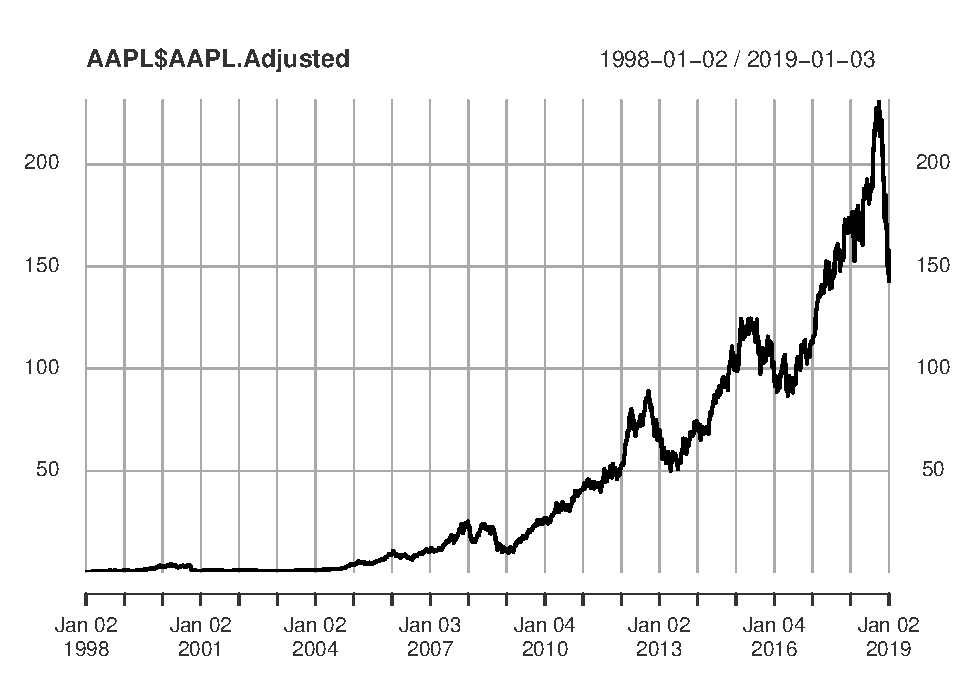
\includegraphics{open-quant-live-book_files/figure-latex/unnamed-chunk-14-1.pdf}

We called the \texttt{quantmod::getSymbols} function with the following
arguments:

\begin{itemize}
\tightlist
\item
  \texttt{Symbols=\textquotesingle{}AAPL\textquotesingle{}} defines a
  character vector specifying the names of each symbol to be loaded,
  here specified by the symbol of the company Apple Inc.;
\item
  \texttt{src="av"} specifies the sourcing method, here defined with the
  value corresponding to Alpha Vantage;
\item
  \texttt{output.size="full"}specified length of the time series
  returned. The strings \texttt{compact} and \texttt{full} are accepted
  with the following specifications: \texttt{compact} returns only the
  latest 100 data points; \texttt{full} returns the full-length time
  series of up to 20 years of historical data;
\item
  \texttt{adjusted=TRUE} defines a boolean variable to include a column
  of closing prices adjusted for dividends and splits;
\item
  \texttt{api.key} specifies your Alpha Vantage API key.
\end{itemize}

\subsection{IEX}\label{iex}

The IEX Group operates the Investors Exchange (IEX), a stock exchange
for U.S. equities that is built for investors and companies. IEX offers
U.S. reference and market data including end-of-day and intraday pricing
data. IEX offers an API with ``a set of services designed for developers
and engineers. It can be used to build high-quality apps and services''.
Data sourced from the IEX API is freely available for commercial subject
to \href{https://iextrading.com/api-exhibit-a/}{conditions} and the use
of their API is subject to additional
\href{https://iextrading.com/api-terms/}{terms of use}.

IEX lists the following github project as an unofficial API for R:
\url{https://github.com/imanuelcostigan/iex}. We will provide examples
on how to obtain intraday pricing data using this package. First, we
will use the \textbf{devtools} to install the package directly from its
github repository as follows:

\begin{Shaded}
\begin{Highlighting}[]
\KeywordTok{library}\NormalTok{(devtools)}
\KeywordTok{install_github}\NormalTok{(}\StringTok{"imanuelcostigan/iex"}\NormalTok{)}
\end{Highlighting}
\end{Shaded}

The \textbf{iex} package provides 4 set of functions as follows:

\begin{itemize}
\tightlist
\item
  \texttt{last}: Provides IEX near real time last sale price, size and
  time. Last is ideal for developers that need a lightweight stock
  quote. \href{https://iextrading.com/developer/docs/\#last}{IEX API
  real time API documentation}.
\item
  \texttt{market}: Provides exchange trade volume data in near real
  time. \href{https://iextrading.com/developer/\#market-market}{IEX
  market API documentation}.
\item
  \texttt{stats}: A set of functions that return trading statistics.
  \href{https://iextrading.com/developer/\#stats}{IEX stats API
  documentation}.
\item
  \texttt{tops}: Provides IEX's aggregated bid and offer position in
  near real time for all securities on IEX's displayed limit order book.
  \href{https://iextrading.com/developer/\#tops-tops}{IEX API TOPS
  documentation}.
\end{itemize}

For instance, the \texttt{last} function has the following arguments:

\begin{itemize}
\tightlist
\item
  \texttt{symbols}: A vector of tickers (case insensitive). Special
  characters will be escaped. A list of eligible symbols is
  \href{https://iextrading.com/trading/eligible-symbols/}{published
  daily} by the IEX. When set to \texttt{NULL} (default) returns values
  for all symbols.
\item
  \texttt{fields}: A vector of fields names to return (case sensitive).
  When set to \texttt{NULL} (default) returns values for all fields.
\item
  \texttt{version}: The API version number, which is used to define the
  API URL.
\end{itemize}

We can obtain intraday stock price data with the \texttt{last} function
as follows:

\begin{Shaded}
\begin{Highlighting}[]
\NormalTok{dat <-}\StringTok{ }\NormalTok{iex}\OperatorTok{::}\KeywordTok{last}\NormalTok{(}\DataTypeTok{symbols =} \KeywordTok{c}\NormalTok{(}\StringTok{"AAPL"}\NormalTok{), }\DataTypeTok{fields =} \KeywordTok{c}\NormalTok{(}\StringTok{"symbol"}\NormalTok{, }
  \StringTok{"price"}\NormalTok{, }\StringTok{"size"}\NormalTok{))}
\end{Highlighting}
\end{Shaded}

The function returns an S3 object of class \texttt{iex\_api} which has
three accessible fields: \texttt{path} , \texttt{response} and
\texttt{content}.

\begin{itemize}
\tightlist
\item
  The \texttt{path} contains the corresponding IEX API path:
\end{itemize}

\begin{Shaded}
\begin{Highlighting}[]
\NormalTok{dat}\OperatorTok{$}\NormalTok{path}
\end{Highlighting}
\end{Shaded}

\begin{verbatim}
## [1] "tops/last"
\end{verbatim}

\begin{itemize}
\tightlist
\item
  The \texttt{response} contains the unparsed IEX API response:
\end{itemize}

\begin{Shaded}
\begin{Highlighting}[]
\NormalTok{dat}\OperatorTok{$}\NormalTok{response}
\end{Highlighting}
\end{Shaded}

\begin{verbatim}
## Response [https://api.iextrading.com/1.0/tops/last?symbols=AAPL&filter=symbol%2Cprice%2Csize]
##   Date: 2019-01-04 06:53
##   Status: 200
##   Content-Type: application/json; charset=utf-8
##   Size: 45 B
\end{verbatim}

\begin{itemize}
\tightlist
\item
  The \texttt{content} contains the parsed content from the API's
  response (usually being a list).
\end{itemize}

\begin{Shaded}
\begin{Highlighting}[]
\NormalTok{dat}\OperatorTok{$}\NormalTok{content}
\end{Highlighting}
\end{Shaded}

\begin{verbatim}
## [[1]]
## [[1]]$symbol
## [1] "AAPL"
## 
## [[1]]$price
## [1] 142
## 
## [[1]]$size
## [1] 100
\end{verbatim}

According to the developer, this package causes R to pause 0.2 seconds
after executing an API call to avoid the user being throttled by the IEX
API (which enforces a 5 request per second limit). Documentation about
the other set of functions can be obtained at
\url{https://github.com/imanuelcostigan/iex/tree/master/man}.

\subsection{Quandl}\label{quandl}

\chapter{Stylized Facts}\label{stylized-facts}

\section{Introduction}\label{introduction}

\section{Distribution of Returns}\label{distribution-of-returns}

\subsection{Fat Tails}\label{fat-tails}

A distribuição de retornos financeiros apresenta leptokurtose. A
ocorrência de eventos extremos é mais provável comparado com uma
distribuição normal, i.e., as caudas da distribuição empírica de
retornos são mais ``pesadas'' comparadas com as caudas esperadas supondo
uma distribuição normal de probabilidade.

\subsection{Skewness}\label{skewness}

A distribuição empírica de retornos é distorcida para esquerda. Retornos
negativos são mais prováveis que retornos positivos.

\section{Volatility}\label{volatility}

\begin{equation}
 \sigma = \sqrt{ \frac{1}{N-1} \sum_{i=1}^N (x_i - \overline{x})^2}
\label{eq:sd}
\end{equation}

\subsection{Time-invariance}\label{time-invariance}

A volatilidade de retornos financeiros não é constante ao longo do
tempo.

\subsection{Volatility Clustering}\label{volatility-clustering}

Eventos extremos são observados próximos um dos outros.

\subsection{Correlation with Trading
Volume}\label{correlation-with-trading-volume}

O volume de negociação de um ativo tem correlação significante com a
volatilidade do mesmo.

\section{Correlation}\label{correlation}

\begin{equation}
\label{eq:correlation}
\rho = \frac{\sum\limits_{t=1}^{T} (r_t - \hat{r}_t)(s_t - \hat{s}_t)}{\sqrt{\sum\limits_{t=1}^{T} (r_t^{\tau} - \hat{r}_t^{\tau})^2}\sqrt{\sum\limits_{t=1}^{T}(s_t - \hat{s}_t)^2}},
\end{equation}

onde \(\hat{r}_t\) e \(\hat{s}_t\) são a média amostral de \(r_t\) e
\(s_t\), respectivamente.

\subsection{Time-invariance}\label{time-invariance-1}

A correlação entre duas series temporais de retornos financeiros não é
constante ao longo do tempo.

\subsection{Auto-correlation}\label{auto-correlation}

Retornos financeiros apresentam baixa autocorrelação (linear), exceto em
escalas de tempo muito baixas, e.g., minutos, onde há presença de
efeitos de microstructura. Por outro lado, a função de autocorrelação do
valor absoluto de retornos financeiros decai lentamente com o tempo.

A correlação contemporânea é maior do que a correlação cruzada.

\chapter{Correlation \& Causation}\label{correlation-causation}

\part{Algo Trading}\label{part-algo-trading}

\chapter{Limit Order}\label{limit-order}

\part{Portfolio
Optimization}\label{part-portfolio-optimization}

\part{Machine Learning}\label{part-machine-learning}

\part{Econophysics}\label{part-econophysics}

\chapter{Entropy}\label{entropy}

\chapter{Transfer Entropy}\label{transfer-entropy}

\chapter{Financial Networks}\label{financial-networks}

\bibliography{book.bib,packages.bib}

\end{document}
